\documentclass{article}
% Margin definition.
\usepackage[a4paper,total={6.8in, 8.5in}]{geometry}
\usepackage{parskip}
% Images.
\usepackage{graphicx}
\usepackage[hidelinks, bookmarks=true]{hyperref}
\usepackage{float}
% Encoding.
\usepackage[english]{babel}
\usepackage[utf8]{inputenc}
\usepackage{epigraph}
% Allow multiline comments
\usepackage{verbatim} 
% To have another layer of sub sections - \paragraph
\usepackage{titlesec}

\setcounter{secnumdepth}{4}

\titleformat{\paragraph}
{\normalfont\normalsize\bfseries}{\theparagraph}{1em}{}
\titlespacing*{\paragraph}
{0pt}{3.25ex plus 1ex minus .2ex}{1.5ex plus .2ex}
% Helvetic font.
\usepackage[scaled]{helvet}
\renewcommand\familydefault{\sfdefault} 
% Header for UA logo.
\usepackage{fancyhdr}
% package for plots / graphics
\usepackage{pgfplots}
\pgfplotsset{width=10cm,compat=newest}
% Dots in index.
\usepackage[titles]{tocloft}
\renewcommand{\cftsubsecleader}{\Large\cftdotfill{0}}
\renewcommand{\cftsecleader}{\Large\cftdotfill{0}}
\renewcommand{\cftsecfont}{\large\bfseries\scshape}
\renewcommand{\cftsubsecfont}{\scshape}
\renewcommand*{\HyperDestNameFilter}[1]{\jobname-#1}
% Dot after number in (sub)sections and in toc.
\renewcommand{\cftsecaftersnum}{.}
\renewcommand{\cftsubsecaftersnum}{.}
\usepackage{titlesec}
\titlelabel{\hspace{-0.5cm}\quad}
\usepackage[letterspace=45]{microtype}
\newcommand*{\fullref}[1]{\hyperref[{#1}]{\autoref*{#1} \nameref*{#1}}}
% Header with UA logo definition. 
\pagestyle{fancy}
\fancyhf{}
\chead{
    
\includegraphics[width=5in]{./images/header_ua.png}
}
\setlength\headheight{20pt}
% Footer with page number.
\rfoot{Page \thepage}
\renewcommand{\footrulewidth}{0.1pt}
% Rename table of contents title to "Index"
\renewcommand{\contentsname}{\normalsize Index \vspace{0.6cm}}
% Add text with hyperlink
\usepackage{hyperref}
%\hypersetup{
%    colorlinks=true,
%    linkcolor=blue,
%    filecolor=magenta
%}
% Water mark
\newsavebox\mybox
\usepackage[printwatermark]{xwatermark}
\usepackage{xcolor}
\usepackage{tikz}
% paragraph
\newcommand\tab[1][1cm]{\hspace*{#1}}
\setlength\parindent{24pt}
%images
 \usepackage{graphicx}
\usepackage{caption}
% footnotes at bottom
\usepackage[bottom]{footmisc}
% Urls with line break
\usepackage{pdflscape}
% Drawing functions
\usepackage{tikz}
\usepackage{pgfplots}
\pgfplotsset{width=7cm, height=4cm, compat=1.17}

\usepackage{multicol}
\setlength{\columnsep}{1cm}

%%%%%%%%%%%% References/Bibliography %%%%%%%%%%%%
\usepackage{biblatex}
\addbibresource{bibliography.bib}

%%%%%%%%%%%%%%%%%%%%%%%%%%%%%%%%%%%%%%%%%%%%%%%%%

\begin{document}

%%%%%%%%%%%%%%%%%% Cover Page %%%%%%%%%%%%%%%%%%
\title{\vspace{-0.9cm}
       \vspace{1cm}
       \normalsize
       \raggedright\textbf{Title: \hspace{1.5cm} Bitcoin: An Overview} \\ \vspace{0.4cm}
       \raggedright\textbf{Authors: \hspace{0.95cm} Eduardo Santos, Hugo Ferreira, João Soares, Pedro Bastos} \\ \vspace{0.4cm}
       \raggedright\textbf{Date: \hspace{1.45cm} 13/04/2021} \\}
\author{}
\date{}

\maketitle
\thispagestyle{fancy}

%%%%%%%%%%%%%%%%%% END Cover Page %%%%%%%%%%%%%%%%%%

\vspace{-1.4cm}

\tableofcontents


\fontsize{10pt}{13pt}
\selectfont
\lsstyle

\titlelabel{\thetitle.\quad}	

\newpage

\section{Introductory Note}

\tab This report consists of a brief analysis of Bitcoin and its protocol, exploring its surge and growth in the cryptocurrency market.
We will also address the topic of Blockchain, and how does it work.

\section{Summary / Abstract}

\tab Bitcoin is a cryptocurrency that has been widely spoken over the past few years, majorly because of what it represents: the beginning if the globalization of digital currencies.

\section{Cryptocurrencies}

\section{Blockchain}

\subsection{What is the Blockchain?}

\subsection{How does it work?}

\section{Bitcoin}

\subsection{What is Bitcoin?}

\subsection{The Seven Pillars of Bitcoin}

\tab The Bitcoin system has seven main pillars that allow the construction of a fair market. 

%Added [H] after so that image is placed after the text above
%This is only possible by adding also \usepackage{float} to the preamble
\begin{figure}[H]
    \begin{center}
        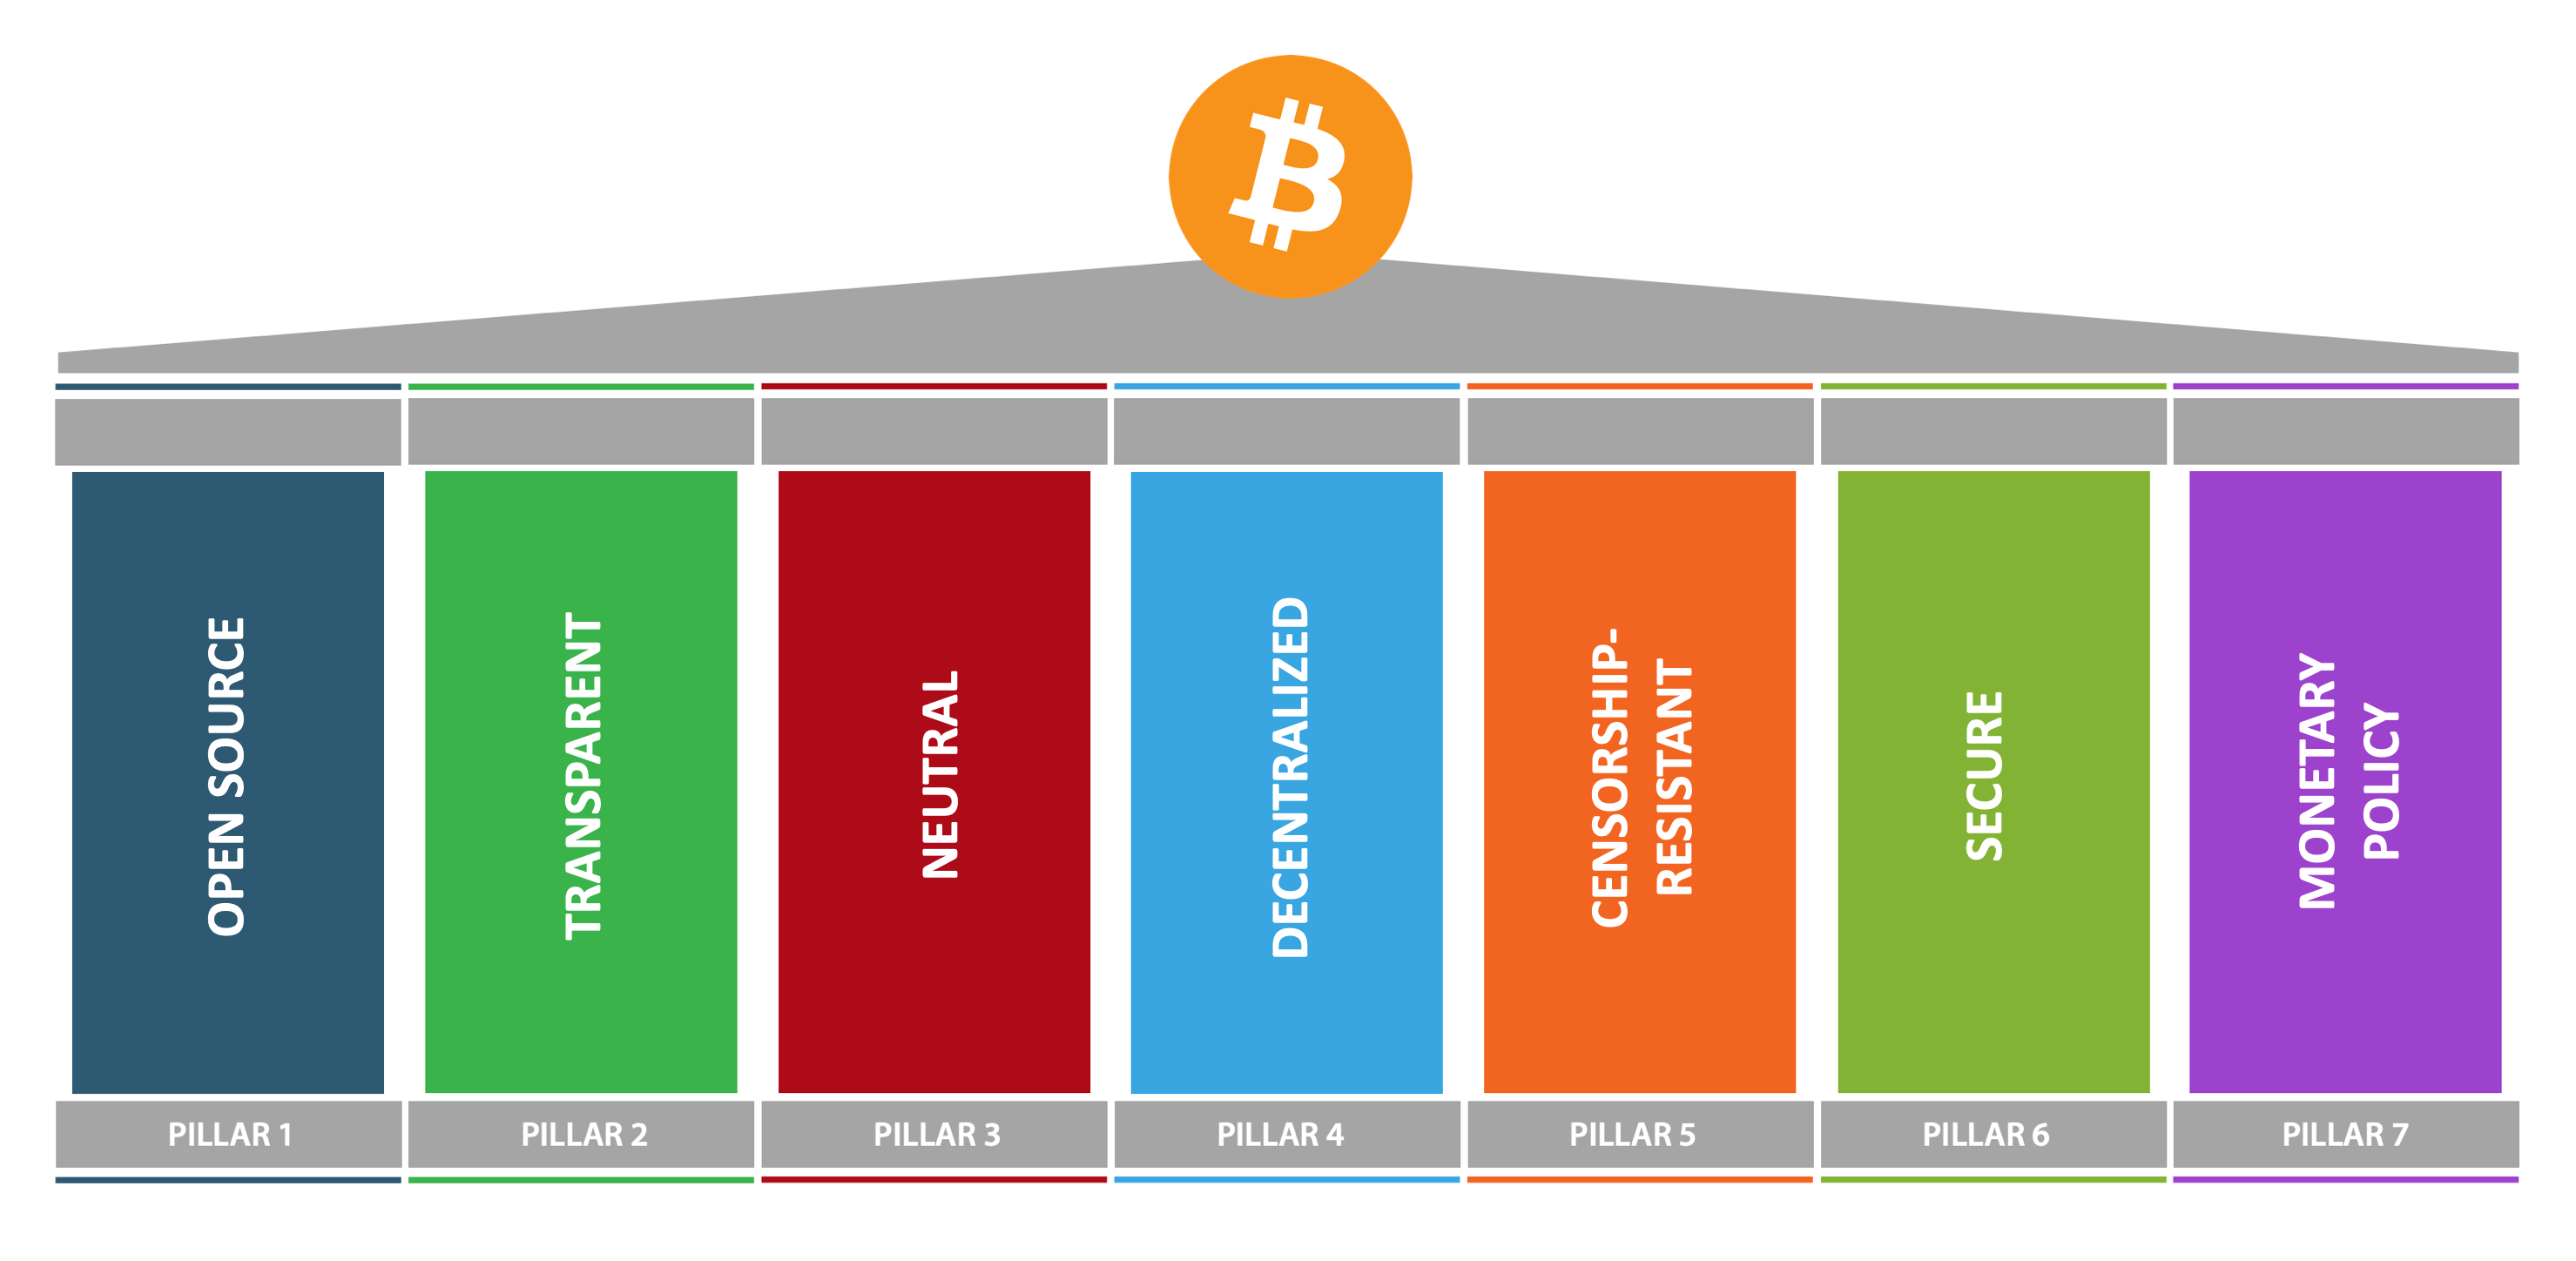
\includegraphics[width=\textwidth]{images/pillars.png}
        \caption{\textit{Pillars of Bitcoin}}
    \end{center}
\end{figure}

\subsubsection{Open Source}

\tab This will be the first pillar approached. Bitcoin is based on the open source software core. This means that the source code is available to anyone who wants to see how the network works. Not only that, anyone can contribute to it. There is a resemblance with the Linux community. The community that daily keeps improving it is its main strength.

With that in mind, bitcoin will not be replaced by a more powerful technology. As mentioned earlier, its developers will keep improving it, making it evolving alongside the internet. Besides that, its security is an essential point to keep improving. And again, thanks to its developers, it will keep up, allowing bitcoin to continue its dominance in the cryptocurrencies market.

\subsubsection{Transparent}

\tab As it was explained in the open source topic, bitcoin blockchain is based on open source code and anyone can check it. Besides that, anyone can enter the network, making bitcoin trustless and permissionless. Anyone can verify any transaction made in the network. This allows people to form their own opinion regarding this market. That is why bitcoin is originally based on a simple quote:

\renewcommand{\epigraphflush}{center}
\epigraph{\textbf{Don't trust, verify.}}{\textit{Bitcoin's motto}}

This is a very important aspect of bitcoin. All users can verify everything by their own, making their decisions a lot easier and allowing them the opportunity to see the impact of every transaction.


\subsubsection{Neutral}

\tab As this system, capable of revolutionizing the current financial system, is available to literally anyone, the success of bitcoin its every user's responsibility. And by this we mean that the users are the ones who make the difference. So, there isn't really an owner of bitcoin. Everyone has equally the same influence. With this, your transactions are only made by you and no one can have a say in it. 

There are many studies that point bitcoin to the U.S dollar's next replacement as the world's reserve currency. They predict the fall of the U.S dollar and the rise of bitcoin, as it is politically neutral. 

%Added [H] after so that image is placed after the text above
%This is only possible by adding also \usepackage{float} to the preamble
\begin{figure}[H]
    \begin{center}
        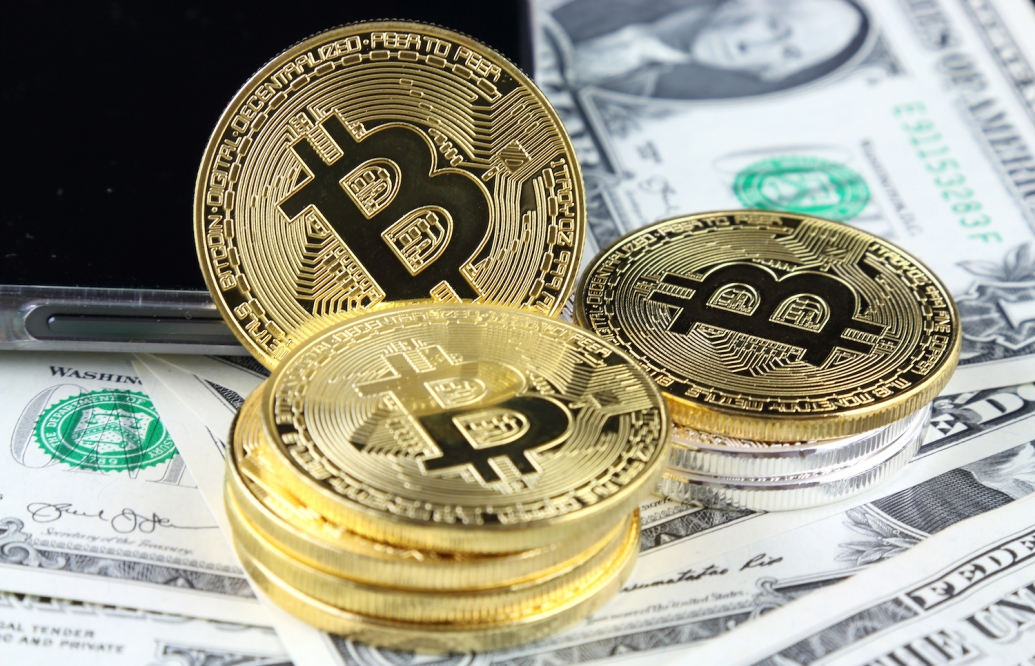
\includegraphics[width=0.5\textwidth]{images/dollar_bitcoin.jpeg}
    \end{center}
\end{figure}

\subsubsection{Decentralized}

\tab The whole bitcoin system is decentralized. This means that it is distributed and resistant to potential attacks. Because of this, its up-time is incredibly high: \textbf{99.985\%}, making it almost unbreakable. 

Bitcoin remains the easiest, fastest and most efficient solution to transfer any amount of money across the world. When compared to other solutions, like banks, its transaction fees and taxes are almost insignificant. In addition, the transaction time is also much faster, completing any transaction in 10 minutes. This is usually 300 times faster than any bank transaction. 

As you probably go to this, it is pretty obvious that bitcoin allows you to make transactions without the inter bank system making it difficult.

\subsubsection{Censorship-Resistant}

\tab As we discussed before, bitcoin has always been a democracy in the sense that there is no leader, all users are equally relevant. Each users possesses their own bitcoins as long as they have their private keys, and no one can take that away. 

\renewcommand{\epigraphflush}{center}
\epigraph{\textbf{Not your keys, not your Bitcoins.}}{\textit{Bitcoin's rules}}

Therefore, you have no fear that your bitcoins will be confiscated by any government. This is a major guarantee that you can have by owning bitcoins.

\subsubsection{Secure}

\tab Bitcoin miners are responsible for validating blocks of transactions by allowing their own computing power to be used by the network. To ensure that these miners run the operation smoothly, they are rewarded by 2 things:

\begin{itemize}
    \item \textbf{Halving - Bitcoin reward every 210,000 blocks issued}
    \item \textbf{Transaction fees}
\end{itemize}

 Currently, this makes bitcoin the most secure network in the entire world. 
 
\subsubsection{Monetary Policy}

\tab The bitcoin's policy will prevent bitcoin from its vanishment. Unlike the U.S dollar, bitcoin exists in limited amounts, as there will be no more than 21 million BTC\footnote{Bitcoins} in circulation. This ensures users that they always own the same percentage of the world's bitcoins as time goes by.

In addition, the process of creating new bitcoins is always predictable. No one can change it and everyone can know when new bitcoin will be created, as it is not influenced by any human decision. 

This makes bitcoin's policy better than the one practiced by the banks. The banks' policies change the money quantity and this is not a problem with bitcoin.




\subsection{The Bitcoin Protocol}

\tab Being a decentralized digital currency, Bitcoin is not something that we can physically own, which in itself generates a large deviation from the concept of money that we are used to and that we use in our day-to-day. To use this digital asset, there are many steps/rules that need to be followed, they make up the Bitcoin protocol.

Bitcoins are not stored centrally nor locally, they exist in a distributed ledger called blockchain. This ledger runs on a P2P\footnote{peer-to-peer} network of computers. 

Owning a Bitcoin is, nothing more, nothing less than simply having the power to transfer it to someone else, with the transaction being recorded in the blockchain. But how does this work?

This is made possible with the usage of an private key - public key ECDSA\footnote{Elliptic Curve Digital Signature Algorithm} pair.

\subsubsection{ECDSA}

\tab ECDSA is a variant of the DSA\footnote{Digital Signature Algorithm}, this uses elliptic curve cryptography. An elliptic curve is mathematically represented by the following equation:

\[y^2 = ax^3 + bx + c\]

In the case of Bitcoin:

\[a = 1\]
\[b = 0\]
\[c = d\: mod\: p\]
\[d = 7\]
\[p = 1.158 \times 10^{77}\]

Replacing the values, we obtain:

\[y^2 = x^3 + 7 \bmod{1.158 \times 10^{77}}\]

Finally, this equation can be translated to the following graphic:

\vspace{5mm} %5mm vertical space

%Added [H] after so that image is placed after the text above
%This is only possible by adding also \usepackage{float} to the preamble
\begin{figure}[H]
    \begin{center}
        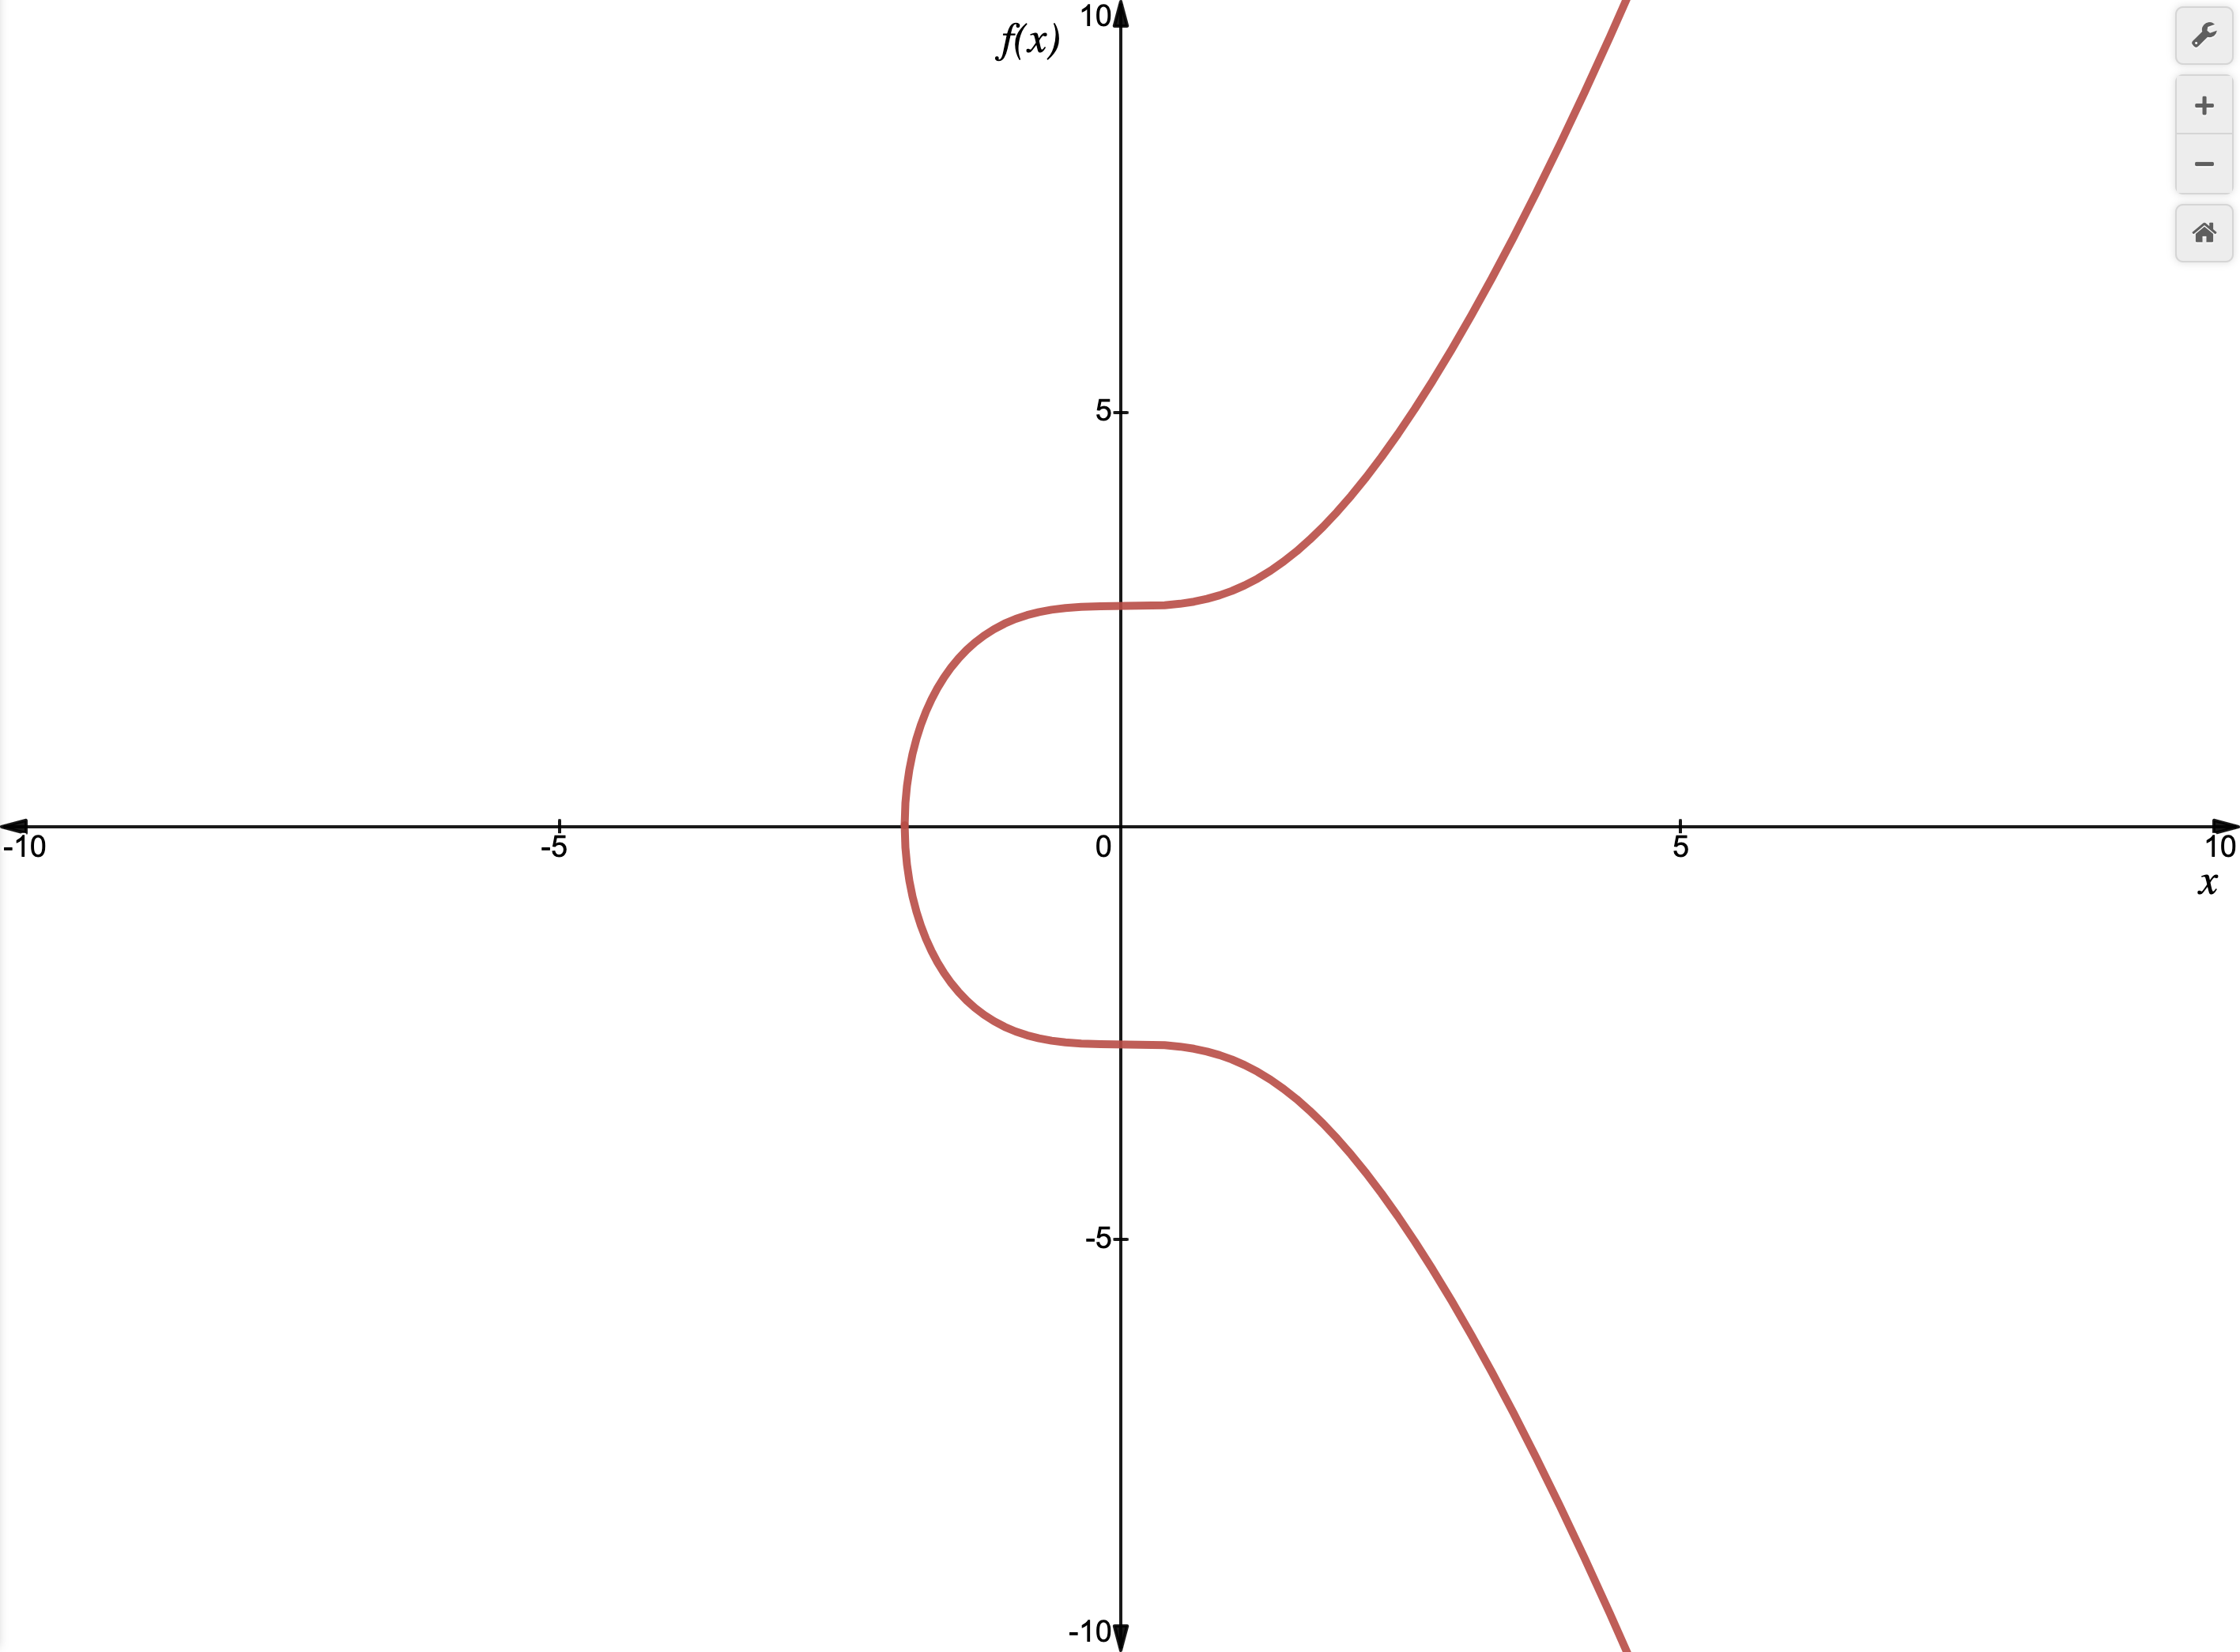
\includegraphics[width=0.6 \textwidth]{images/Kobiltz_curve.png}
        \caption{\textit{Kobiltz curve}}
    \end{center}
\end{figure}

\vspace{5mm} %5mm vertical space

\begin{comment}
%Added [H] after so that image is placed after the text above
%This is only possible by adding also \usepackage{float} to the preamble
\begin{figure}[H]
    \begin{center}
        \begin{tikzpicture}
            \begin{axis}[
                width=0.5\textwidth,
                height=0.3\textwidth,
                xmin=-5,
                xmax=5,
                ymin=-5,
                ymax=5,
                xlabel={$x$},
                ylabel={$f(x)$},
                scale only axis,
                axis lines=middle,
                smooth,
                domain=-1.912931:3, %supostamente, sem esta linha o gráfico divide-se em 2 partes, tristeza
                xtick={-5,...,0,...,5},
                ytick={-5,...,0,...,5},
            ]
                \addplot [red] {sqrt(x^3 + mod(7, 1.158*10^(77)))};
                \addplot [red] {-sqrt(x^3 + mod(7, 1.158*10^(77)))};
            \end{axis}
        \end{tikzpicture}
    \end{center}
    \caption{Kobiltz curve}
\end{figure}
\end{comment}

The curve on the graph above is called \textit{Kobiltz curve}, and its often referred as \textit{secp256k1}. This curve was created on purpose, and with a very defined objective: to increase efficiency in the generation of public and private keys, making the computation of this key pair 30\% faster. But this is not the only thing that differentiates this curve from the rest of the elliptical curves, due to the precision in choosing the values of the constants \(a, b, c\) and \(d\), the probability of having an attack in the process in a way that can compromise it is as small as possible.

Elliptic curves have some properties, in  this case, for example:

\begin{itemize}
    \item A non-vertical line that intersects two non-tangent points on the curve will always intersect a third point on the same curve.
    \item A non-vertical line tangent to the curve at one point will intersect only one other point on the curve.
\end{itemize}

This properties allow us to define two operations: point addition and point doubling.

\paragraph{Point addition}

\tab Point addition consists of following this steps:

\begin{itemize}
    \item Take two points of the elliptic curve, \(P\) and \(Q\).
    \item Pass a line through the previous points.
    \item Mark the point (\(-R\)) from the intersection of the previous line with the curve.
    \item Mirror \(-R\) through the x-axis, obtaining \(R\)
\end{itemize}

This algorithm can be put into the following expression:

\[P + Q = R\]

With \(R\) being the result of the sum of the original points.

Finally, this equation can be translated to the following graphic:

\vspace{5mm} %5mm vertical space

%Added [H] after so that image is placed after the text above
%This is only possible by adding also \usepackage{float} to the preamble
\begin{figure}[H]
    \begin{center}
        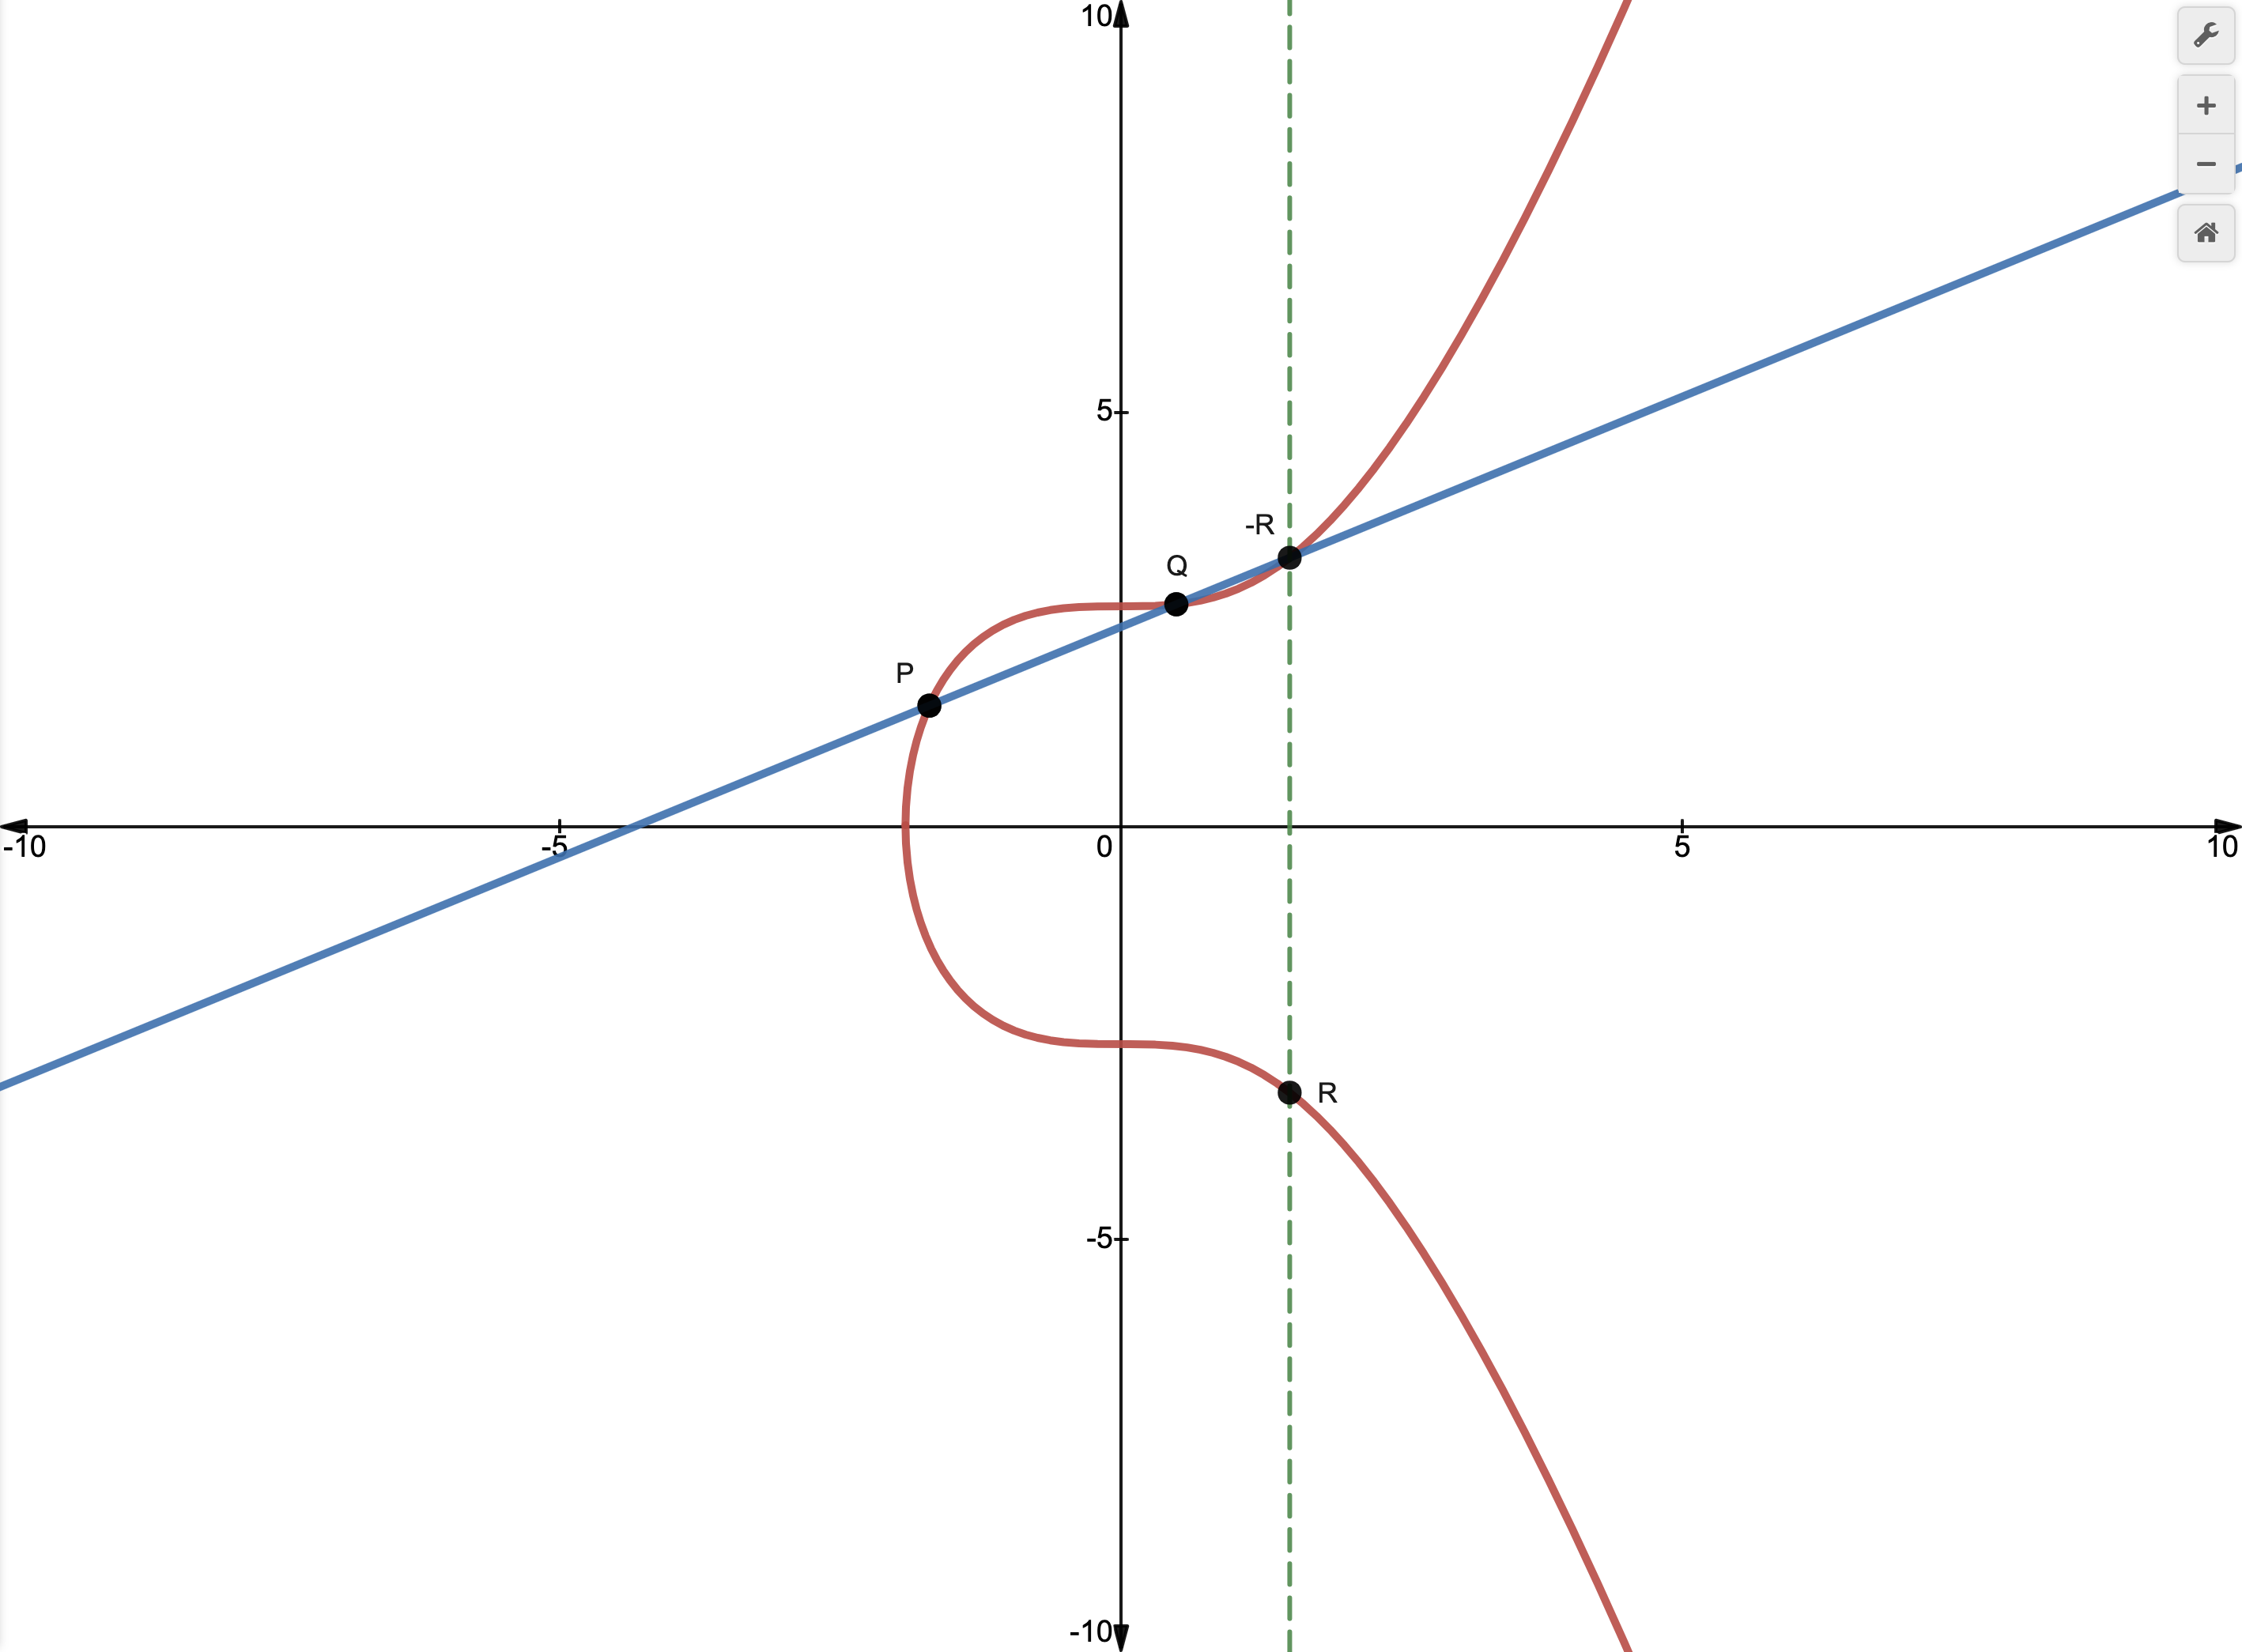
\includegraphics[width=0.6 \textwidth]{images/point_addition.png}
        \caption{\textit{Point addition}}
    \end{center}
\end{figure}

\vspace{5mm} %5mm vertical space

\paragraph{Point doubling}

\tab Point doubling consists of following this steps:

\begin{itemize}
    \item Take a point of the elliptic curve, \(P\).
    \item Pass a tangent line tangent to \(P\).
    \item Mark the point (\(-R\)) from the intersection of the previous line with the curve.
    \item Mirror \(-R\) through the x-axis, obtaining \(R\)
\end{itemize}

This algorithm can be put into the following expression:

\[P + P = 2P = R\]

With \(R\) being the result of the sum of \(R\) with itself.

Finally, this equation can be translated to the following graphic:

\vspace{5mm} %5mm vertical space

\begin{figure}[H]
    \begin{center}
        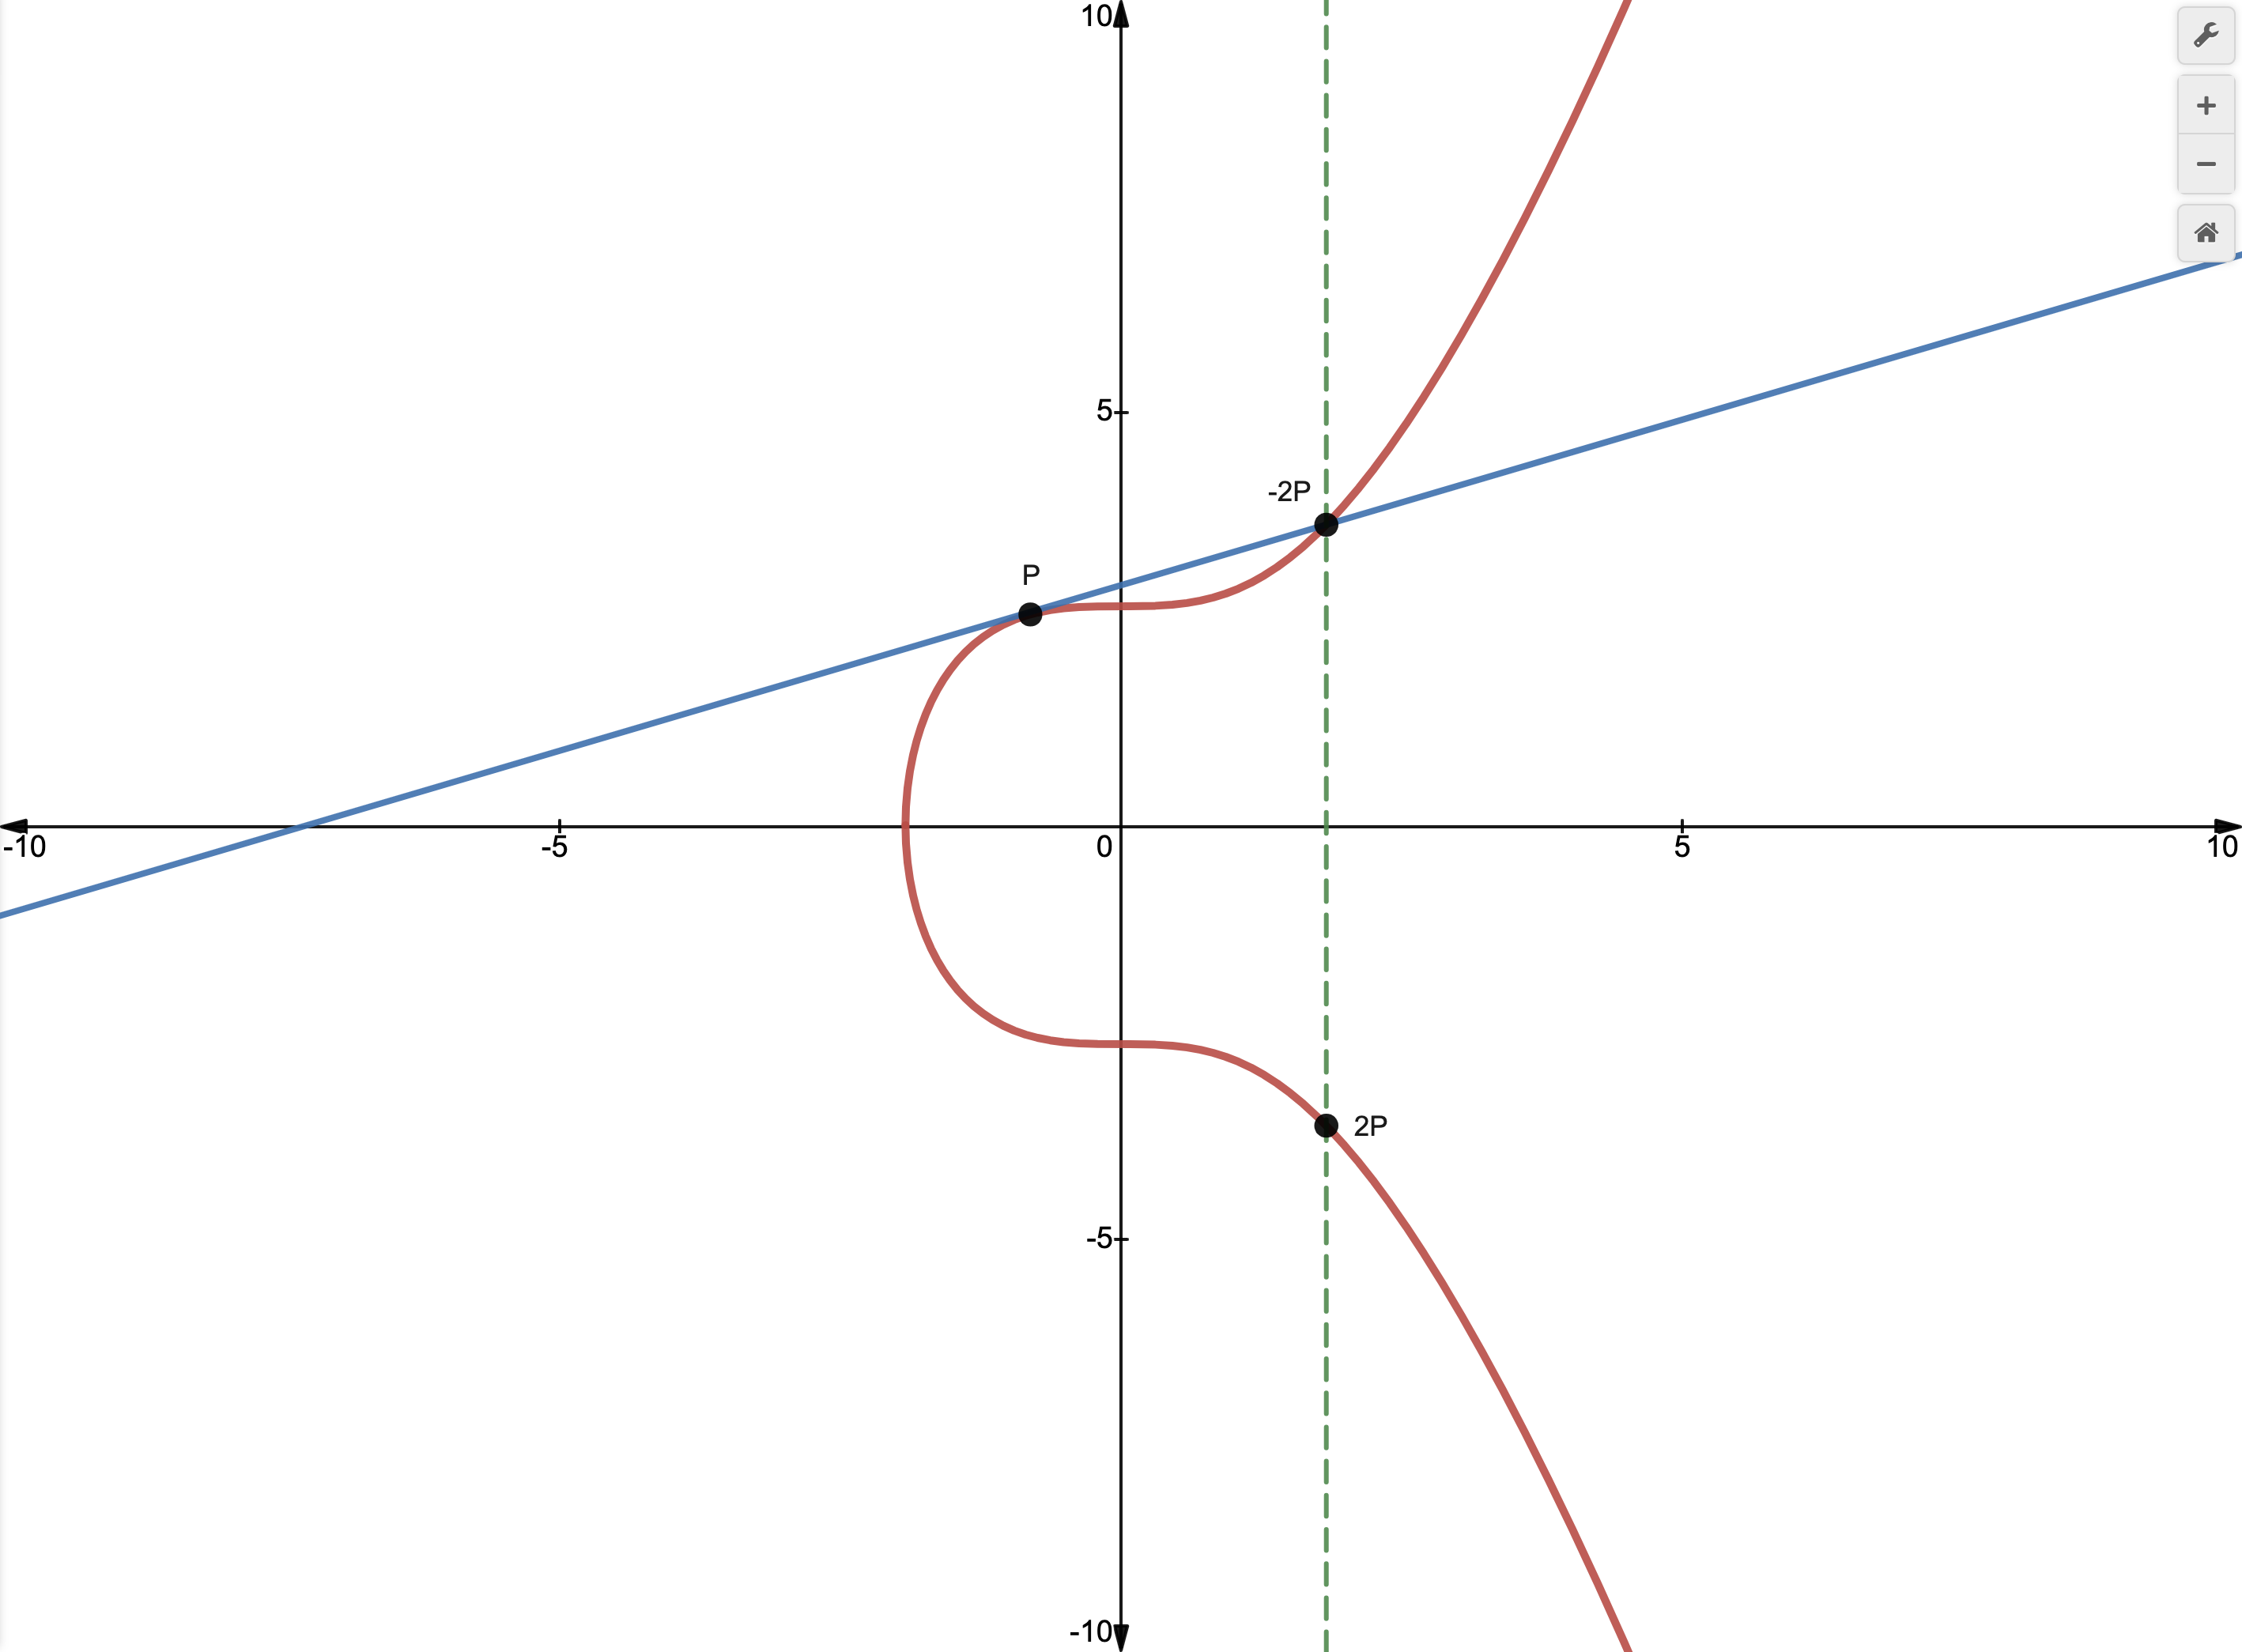
\includegraphics[width=0.6 \textwidth]{images/point_doubling.png}
        \caption{\textit{Point doubling}}
    \end{center}
\end{figure}

\vspace{5mm} %5mm vertical space

\paragraph{Scalar multiplication}

\tab Point addition and point doubling combined are used for scalar multiplication, this means adding a point to itself \(n\) times:

\[R = nP\]

To explain it better, we will use the following example:

\[R = 11P\]
\[R = P + (P + (P + (P + (P + (P + (P + (P + (P + (P + P)))))))))\]

This can be simplified using the previous operations:

\[R = 11P\]
\[R = P + 10P\]
\[R = P + 2(5P)\]
\[R = P + 2(P + 4P)\]
\[R = P + 2(P + 2(2P))\]

As we can see, we just decomposed \(11P\) into two point additions and three point doubling. This can be very useful when \(n\) is a large number.

One of the uses of scalar multiplication is to calculate the private-public key pair, we will take a look on how it works and where it is placed in the Bitcoin protocol in the section bellow.

\subsubsection{Private-Public key pair}

\tab The private-public key pair is used on Bitcoin transactions between users.



\begin{comment}
Graphically is even easier to understand this, for instance, if we take a point \(P\), and we want to obtain \(4P\), the process would result in this graph:

\vspace{5mm} %5mm vertical space

\begin{figure}[H]
    \begin{center}
        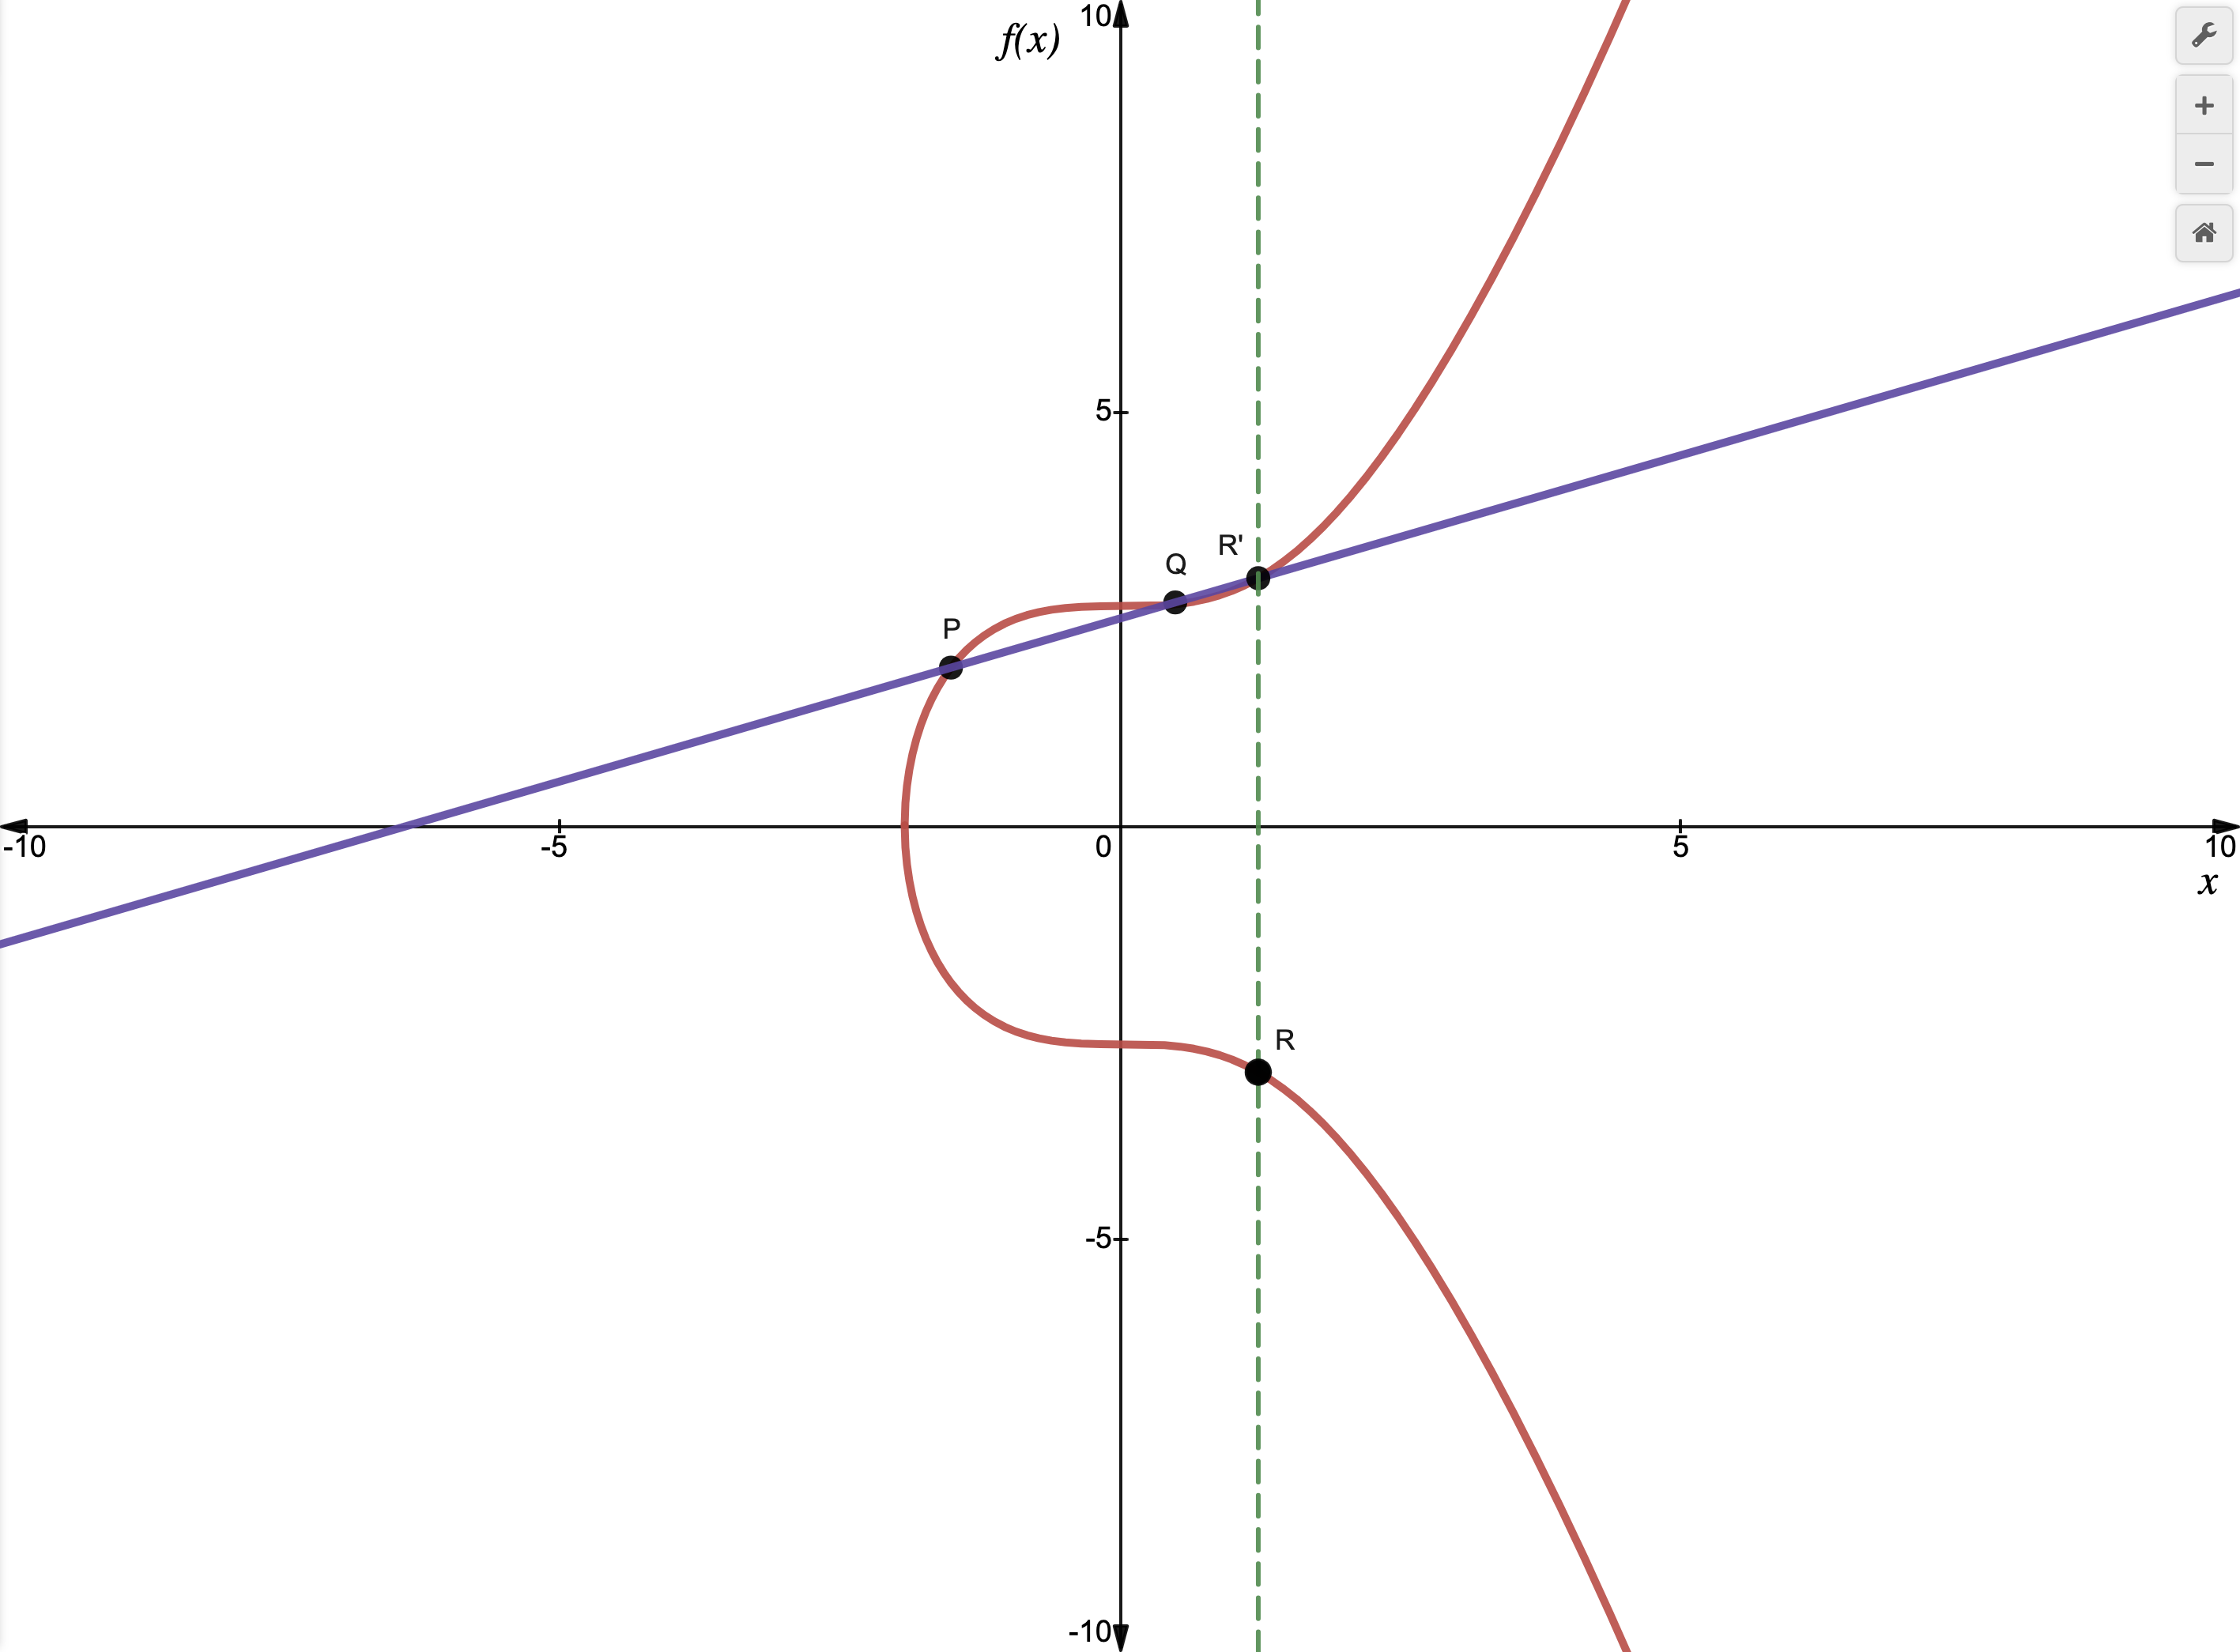
\includegraphics[width=0.6 \textwidth]{images/Kobiltz_curve_with_points.png}
        \caption{\textit{Process of obtaining \(4P\) from the point \(P\), using scalar multiplication}}
    \end{center}
\end{figure}

\vspace{5mm} %5mm vertical space

\end{comment}

%\tab In this case, this pair is used in bitcoin and other cryptocurrencies transactions.

% Add "References" to table of contents
\addcontentsline{toc}{section}{References}
% No cite makes all references appear, even if there's no citation on the text
\nocite{*}
\printbibliography

\end{document}